\documentclass[../tesis_main.text]{subfiles}

%%%%%%%%%%%%%%%%%%%%%%%%%%%%%%%%%%%%%%%
%   Agregar refencias al papper de Justina
%	Describir constitución del robot
%

\chapter{Marco teórico}
	\section{Robots de servicio}
		%Conceptos


		%Estado del arte
		Dado que este trabajo se centrará en los robots de servicio es importante mencionar que un robots de servicio es un robot capaz de realizar tareas de la vida diaria en un ambiente similar al de un hogar real. Actualmente el desarrollo de este tipo de robot está guiado por la comtencia internacional Robocup @Home.\cite{robocupAtHome} Esta categoría promueve la incorporación de habilidades robóticas avanzadas para la interacción con los humanos y con el entorno de operación. Esta competencia se enfoca a desarrollar habilidades en los robots de servicios. Ejemplos de estas habilidades son la localización y navegación segura en ambientes no controlados, la comunicación natural humano-robot por voz y gestos y habilidades visuales para el reconocimiento y la manipulación de objetos.\cite{femexrobotics}\\

		Los robots de servicio enfrentan diversos retos: desarrollar tareas en ámbientes dinámicos, características de entornos no estandarizados, incertidumbre ante escenarios desconocidos. Dadas las condiciones en que estos robots operan los programadores y desarrolladores de robots de servicios han optado por dotar a los robots de ciertas capacidades. Por ejemplo el robot Cosero, consta de un sistema de percepción del entorno, un sistema de manipulación, un sistema de interacción humano-robot y un sistema de planeación de tareas.\\ %%%%REFFFFFF

		\textit{Tabla con las características de los robots de servicio.}\\

		\begin{figure}[htb]
			\begin{center}
			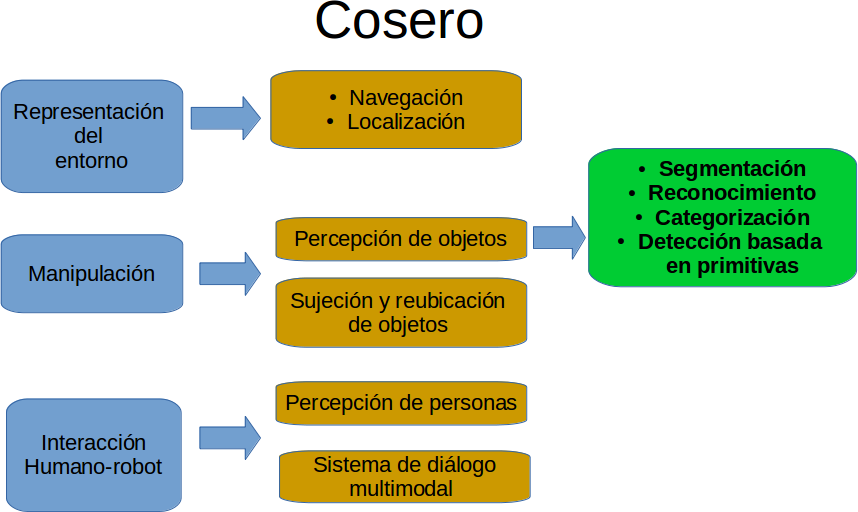
\includegraphics[width=3.5cm, height=5cm]{/cosero.png}
			\caption{Estructura de software del robot Cosero.}
			\end{center}
		\end{figure}

		\begin{figure}[htb]
			\begin{center}
			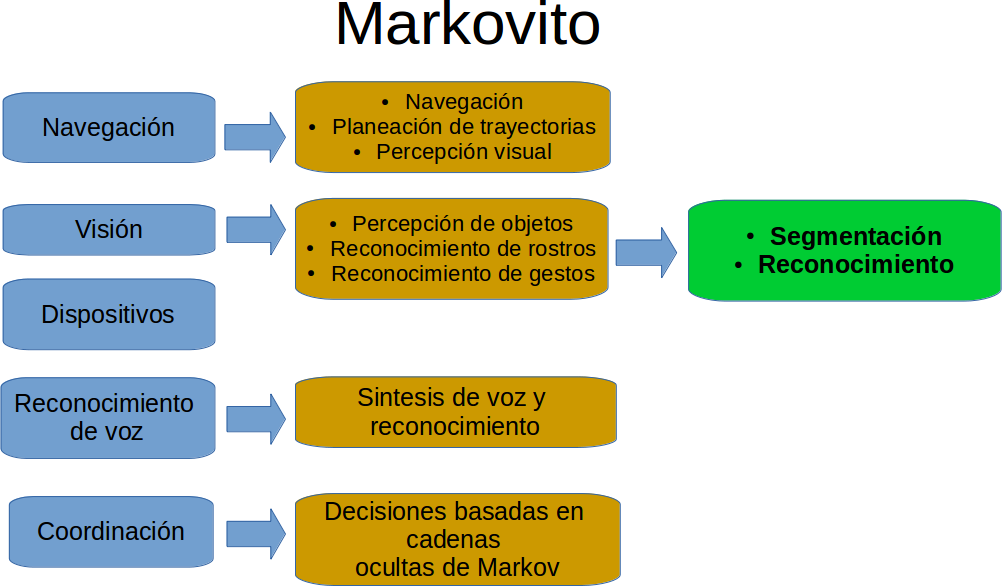
\includegraphics[width=3.5cm, height=5cm]{/markovito.png}
			\caption{Estructura de software del robot Cosero.}
			\end{center}
		\end{figure}

		\begin{figure}[htb]
			\begin{center}
			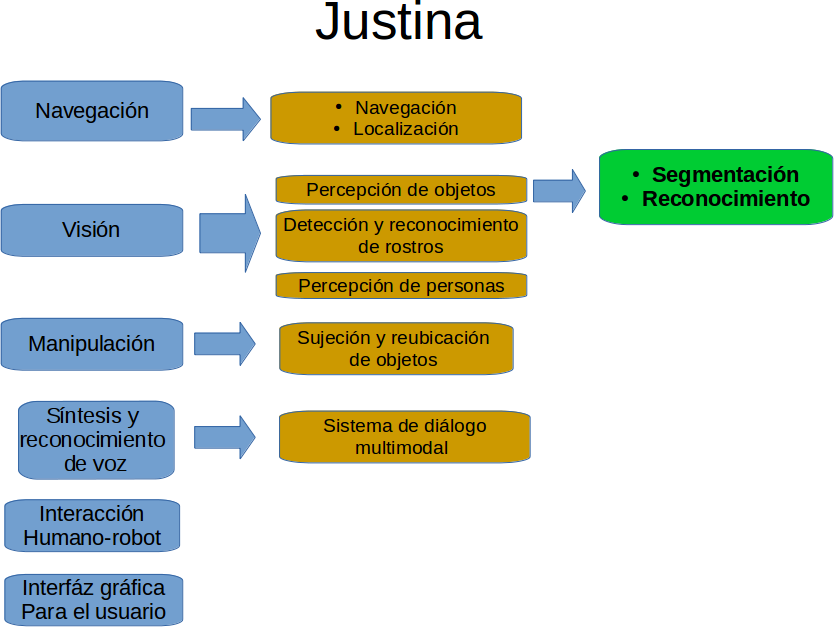
\includegraphics[width=3.5cm, height=5cm]{/justina.png}
			\caption{Estructura de software del robot Cosero.}
			\end{center}
		\end{figure}

		En particular en una metodología de detección y manipulación de objetos, resulta una tarea fundamental a resolver en los robots de servicio. La idea general de la robótica de servicio doméstico ha existido desde hace mucho tiempo, pero es un tema de investigación relativamente joven. El objetivo de crear robots de servicios útiles y autónomos que puedan interactuar con seres humanos y objetos en el mundo real en un entorno natural plantea un gran número de problemas sin resolver en muchas disciplinas científicas.\\
		%\vspace{0.2in}

		Recientemente, el progreso en estos campos de investigación, así como el progreso y la normalización en el desarrollo de hardware y software, ha llevado a un aumento en la disponibilidad de recursos, métodos y componentes para el desarrollo  de Robots de servicio doméstico . Por ello estamos cada vez más cerca de convivir con robots de servicios de manera exitosa en diversos lugares, por ejemplo hospitales \cite{hospitalRobots}, oficinas, construcciones, o tiendas departamentales \cite{robotsInStores}.\\
		%\vspace{0.2in}


		Estos desarrollos han sido posibles gracias a herramientas de código abierto como lo es Ubuntu, ya que ha servido como base para el desarrollo de software especializado para robots, por ejemplo ROS \cite{rosEpage}. Este conjunto de librerías especializadas para robots pueden llegar a ser muy patículares y estar enfocados a una sola área de invetigación de las antes mencionadas, por ejemplo: Carmen \cite{carnegieMellon}, un conjuto de liberías y algoritmos de control para navegación de robots, desarrollados por la universidad Carnegie Mellon\cite{cMellonEpage}.\\
		%\vspace{0.2in}

		En la parte de simulación se cuenta con ejemplos como el USARSim \cite{balakirsky2006}, rviz \cite{rVizEpage} o Gazebo \cite{gazeboEpage}. Por lo que respecta a los algoritmos de visión computacional existen bibliotecas de código abierto por ejemplo OpenCV \cite{openCV} el cual tiene un gran campo de aplicaciones\cite{bradski2000}. Por lo que corresponde a los kits standar de hardware, podemos mencionar la construcción de robots de plataforma standar por ejemplo VolksBot \cite{wisspeintner2007} y las plataformas bases por ejemplo ActivRobots \cite{ActivRobots}, Pepper \cite{pepperEpage}, Asimo \cite{asimoEpage} ha hecho posible desarrollar software de manera más rápida y eficiente.\\
		%\vspace{0.2in}

		\begin{figure}[htb]
			\begin{center}
			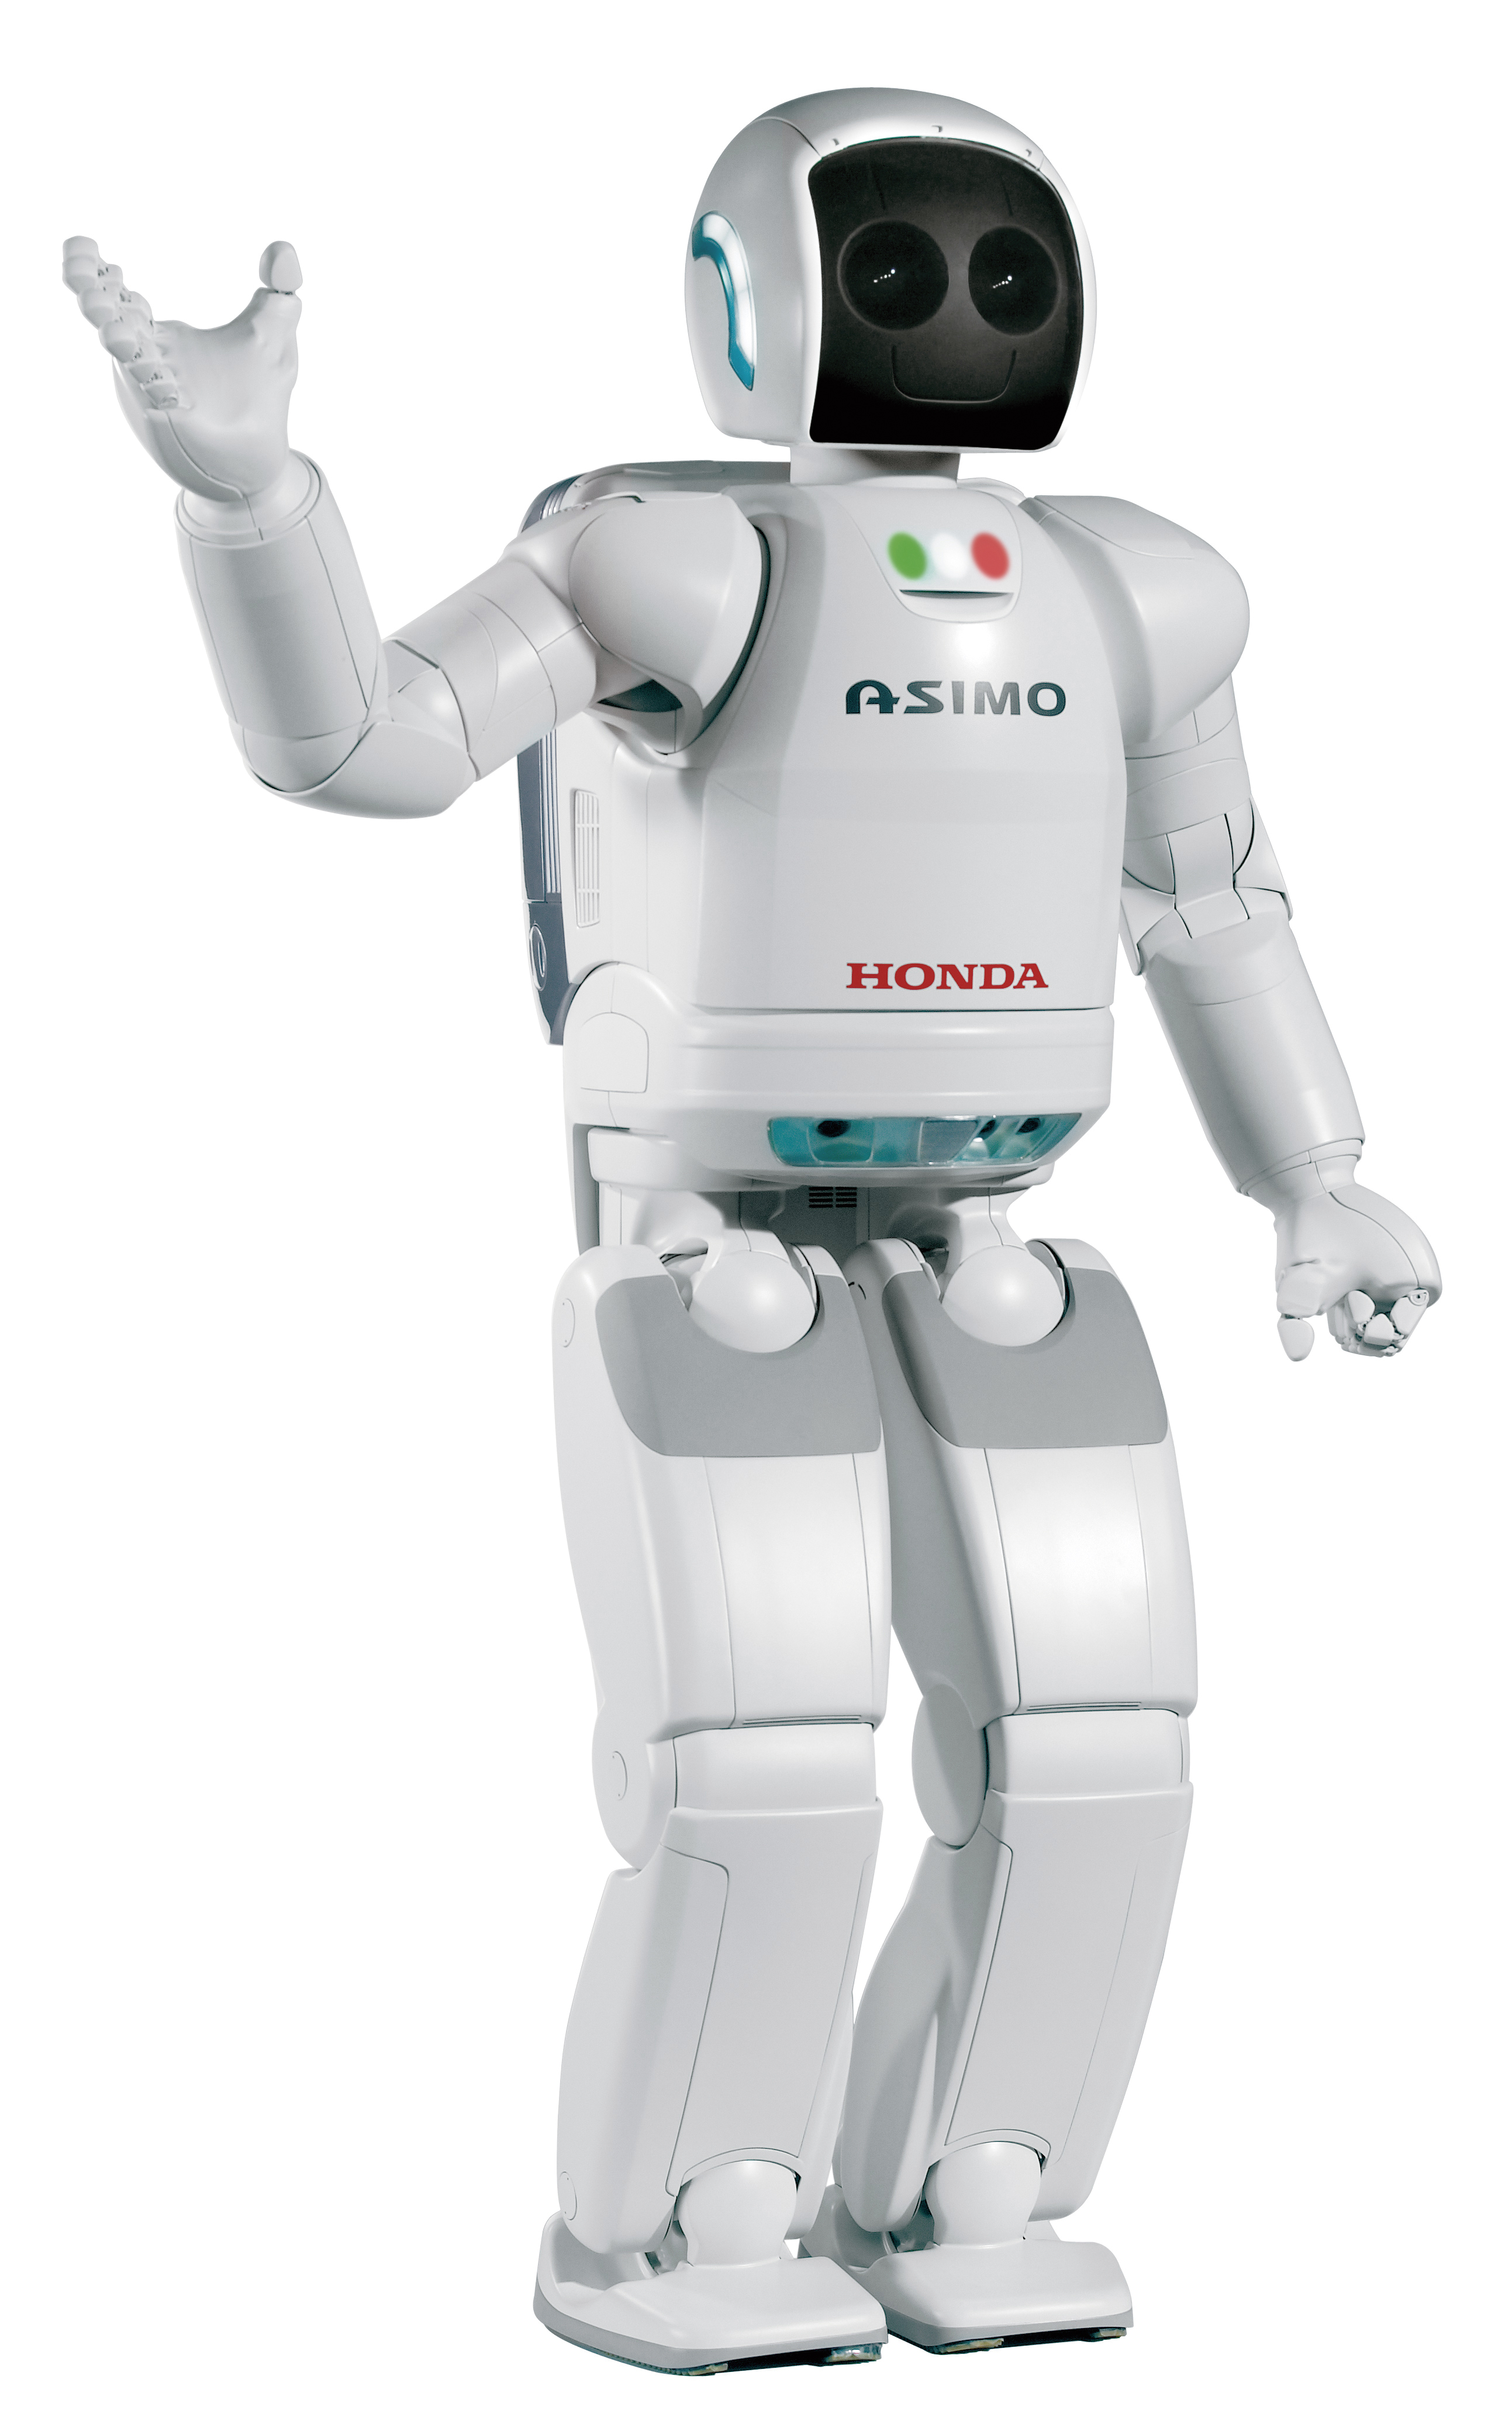
\includegraphics[width=3.5cm, height=5cm]{/asimo.jpg}
			\caption{Robot asimo desarrollado por la companía Honda.}
			\end{center}
		\end{figure}



%%% Fundamentos de Manipuladores
%%  ---------------------------------

	\section{Fundamentos básicos de Robots Manipuladores}
		La manipulación adecuada de objetos es una característica imprescindible en los robots de servicio dadas las condiciones de su entorno y las tareas cotidianas que le podemos asignar a dicho robot. Una posible solución a la problemática de la manipulación de objetos es la incorporación de manipuladores seriales a una base móvil; sin embargo se debe tener encuenta que los objetos a ser manipulados se encuentran en condiciones aleatorias de posición y orientación, estas características implican que el manipulador serial debería ser capaz de alcanzar una posición (x, y, z) con cualquier orientación (roll, pitch, yaw).\\

		Los robots manipuladores clásicos presentan una configuración antropomórfica serial, que hace semejanza con un brazo humano. La arquitectura típica de un manipulador consiste en una serie de barras rígidas unidas entre sí mediante el uso de articulaciones rotacionales o prismáticas. De manera general cada articulación logra su movimiento gracias a un actuador y a la adición de algunos elelmentos complementarios como sensores de posición y de velocidad\cite{baturone2005}.\\

		Los robots manipuladores clásicos están caracterizados, desde el punto de vista mecánico, por una serie de propiedades talez como los grados de libertad, el espacio de trabajo, la rígidez estructural, peso propio y la capacidad de llegar a un punto deseado con exactitud en multiples repeticiones. Además en los robots manipuladores suelen tomarse en cuenta otras características adicionales: la carga útil máxima y la velocidad de trabajo.\\

		\begin{figure}[htb]
			\begin{center}
			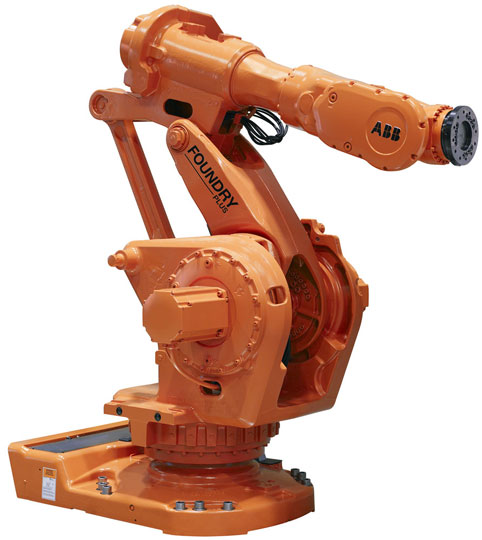
\includegraphics[width=3.5cm, height=4cm]{/serial_abb.jpg}
			\caption{Robot serial elaborado por la companía ABB.}
			\end{center}
		\end{figure}

		\subsection{Configuraciones típicas y parámetros característicos}
			Según la geometría de su estructura mecánica, un manipulador puede ser:

			\begin{itemize}
				\item{Cartesiano, cuyo posicionamiento en el espacio se lleva a cabo mediante articulaciones lineales.}

				\item{Cilíndrico, con una articulación rotacional sobre una base y articulaciones lineales para el movimiento en altura y en radio.}

				\item{Polar, que cuenta con dos articulaciones rotacionales y una lineal.}

				\item{Esférico (o de brazo articulado), con tres articulaciones rotacionales.}

				\item{Mixto, que posee varios tipos de articulaciones, combinaciones de las anteriores. Es destacable la configuración SCARA (Selective Compliance Assembly Robot Arm).}

				\item{Paralelo, posee brazos con articulaciones prismáticas o rotacionales concurrentes. Figura 2.3}
			\end{itemize}

Los principales parámetros que caracterizan a los robots industriales son:

	\begin{itemize}
		\item{Número de grados de libertad. Es el número total de grados de libertad de un robot, dado por la suma de g.d.l. de las articulaciones que lo componen. Aunque la mayoría de las aplicaciones industriales requieren 6 g.d.l., como las de soldadura, mecanizado y almacenamiento, otras más complejas requieren un número mayor, tal es el caso de las labores de montaje.}

		\item{Espacio de accesibilidad o espacio (volumen) de trabajo. Es el conjunto de puntos del espacio accesibles al punto terminal, que depende de la configuración geométrica del manipulador. Un punto del espacio se dice totalmente accesible si el efector final puede situarse en él en todas las orientaciones que permita la constitución del manipulador y se dice parcialmente accesible si es accesible por el efector final pero no en todas las orientaciones posibles. En la figura inferior se aprecia el volumen de trabajo de robots de distintas configuraciones.}

		\item{Capacidad de posicionamiento del punto terminal. Se concreta en tres magnitudes fundamentales: resolución espacial, precisión y repetibilidad, que miden el grado de exactitud en la realización de los movimientos de un manipulador al realizar una tarea programada.}

		\item{Capacidad de carga. Es el peso que puede transportar el elemento terminal del manipulador. Es una de las características que más se tienen en cuenta en la selección de un robot dependiendo de la tarea a la que se destine.}

		\item{Velocidad. Es la máxima velocidad que alcanzan el efector final y las articulaciones.}
	\end{itemize}

		\begin{figure}[htb]
			\begin{center}
			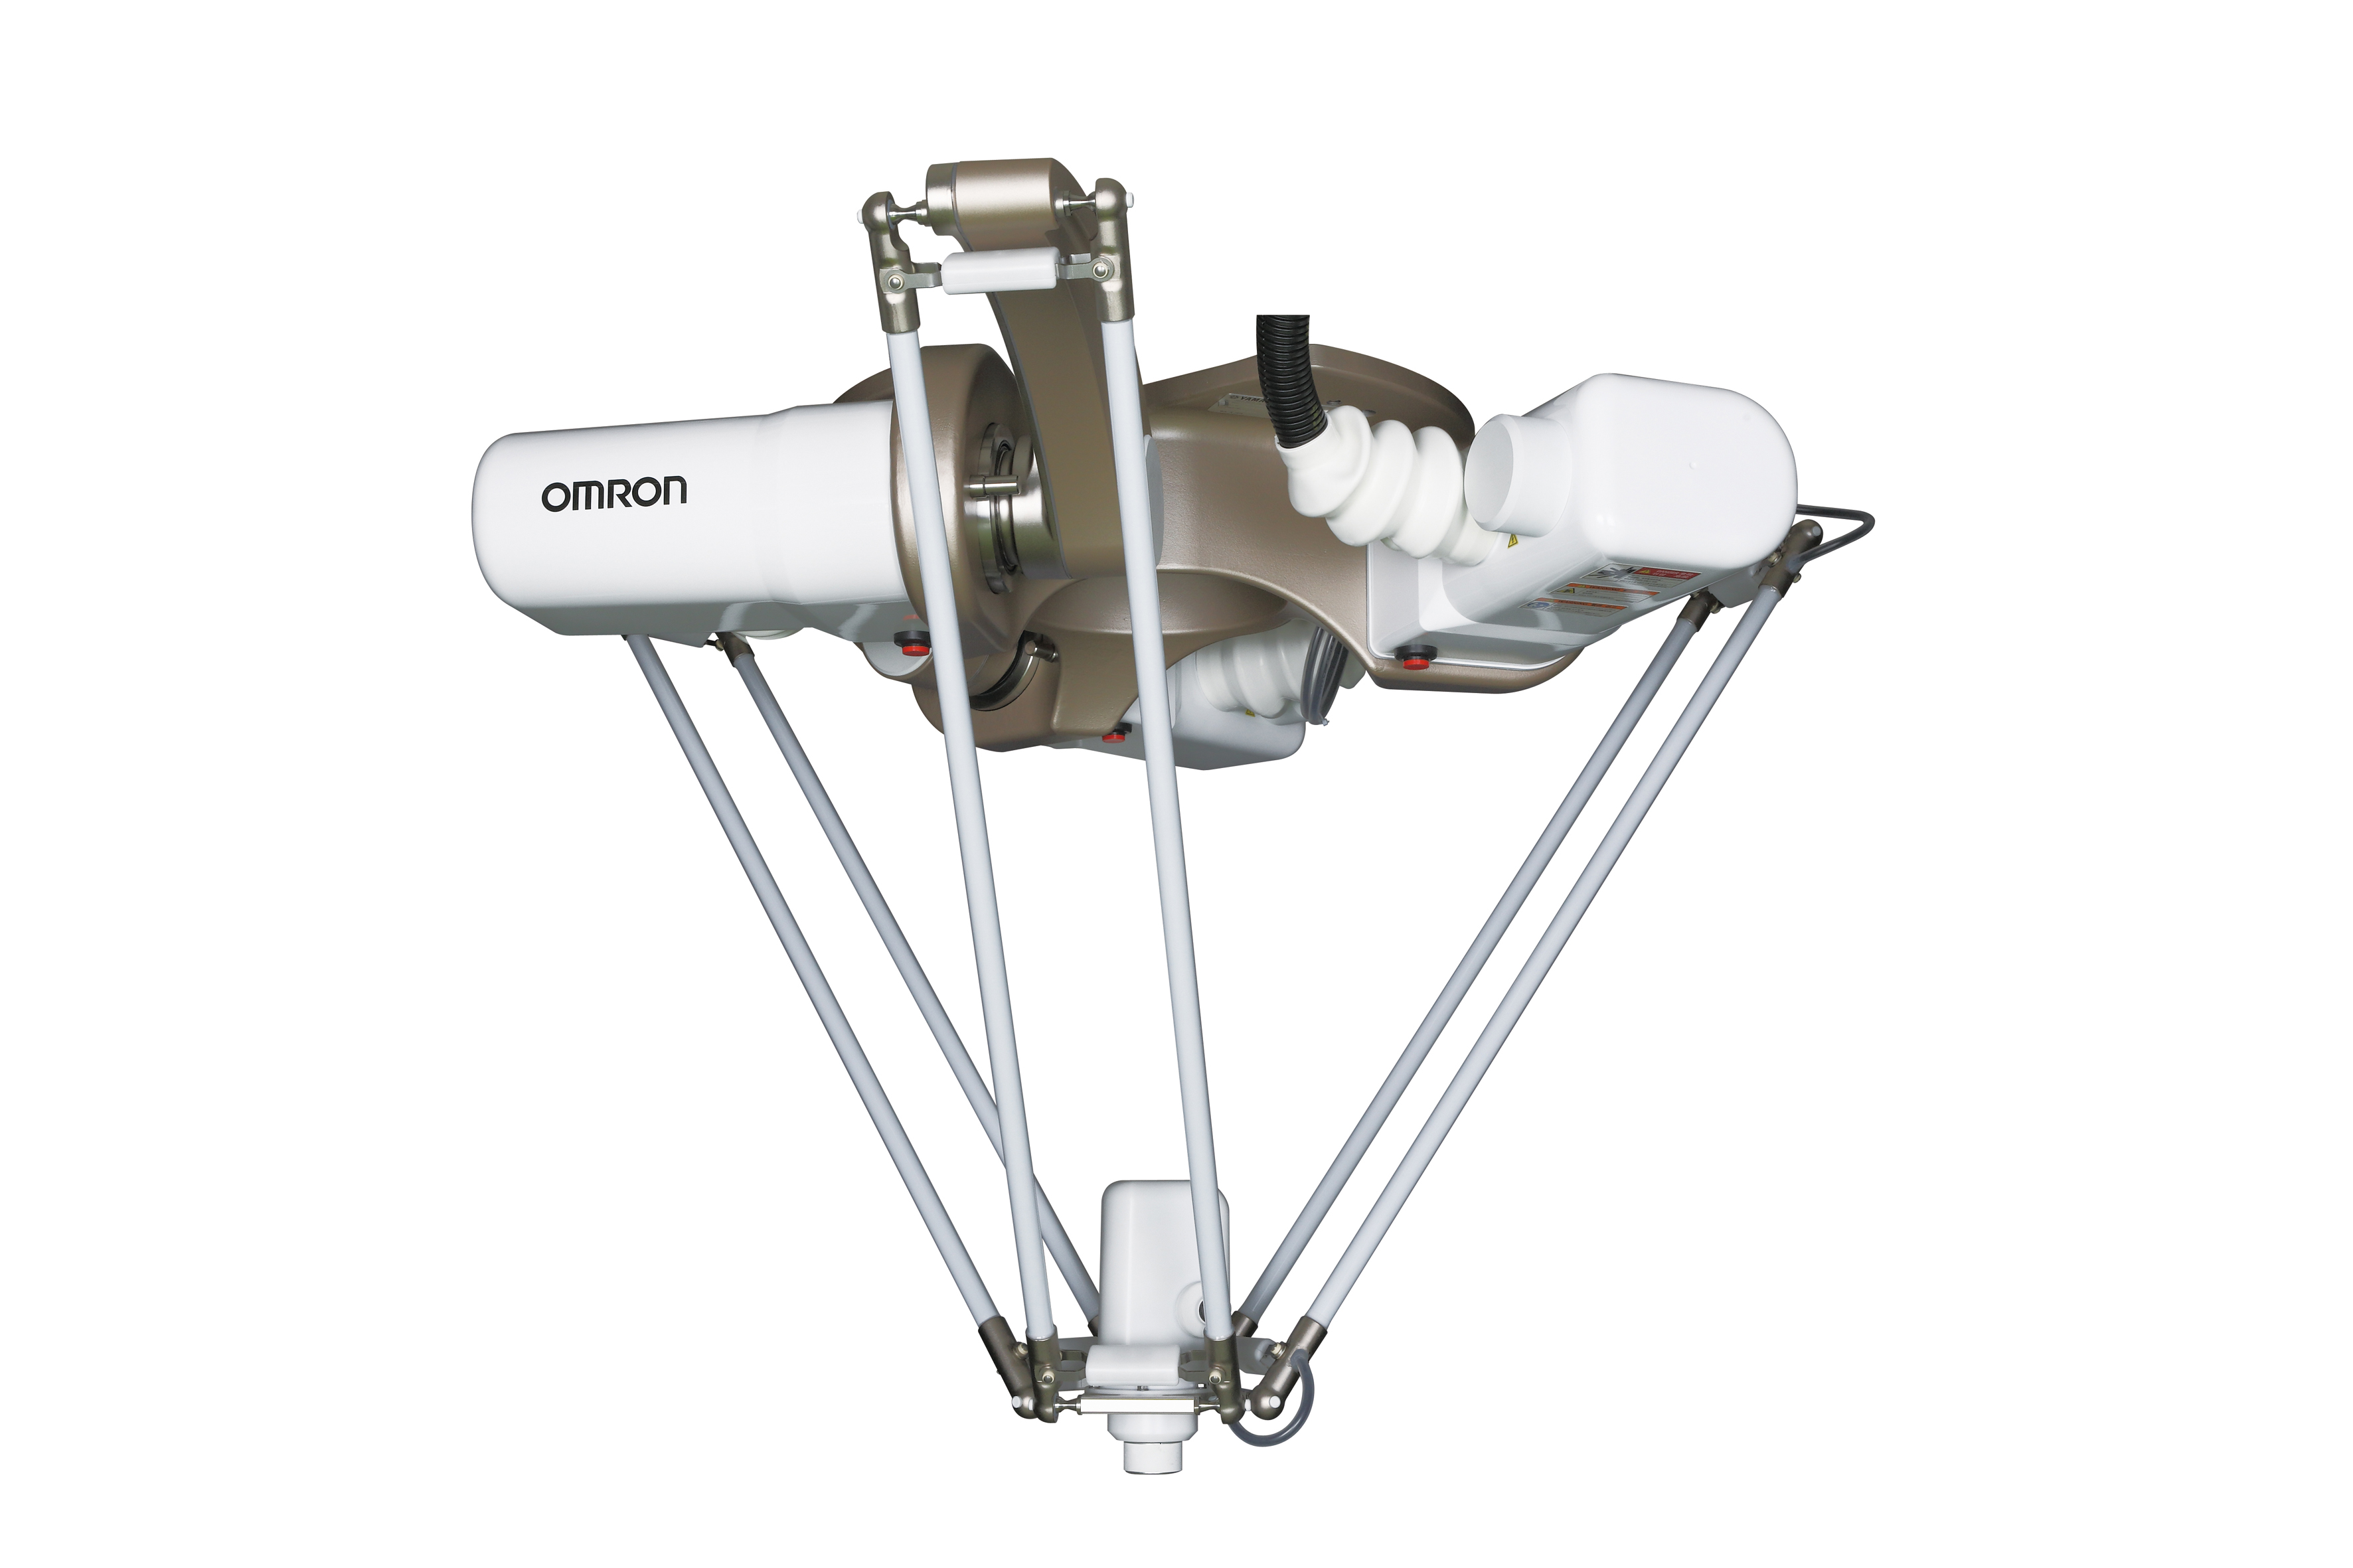
\includegraphics[width=6.5cm, height=4.5cm]{/robotParalelo.jpg}
			\caption{Robot paralelo.}
			\end{center}
		\end{figure}


		\subsection{Descripciones espaciales y transformaciones}
			La cinemática es la ciencia del movimiento que trata el tema sin considerar las fuerzas que lo ocasionan. Dentro de esta ciencia se estudian la posición, la velocidad y la aceleración. En conseciencia, el estudio de la cinemática de manipuladores se refiere a todas las propiedades geométricas y las basadas en los cambios de estas a lo largo del tiempo. Dadas las características de este trabajo solo se abordarán la cinemática directa e inversa, sin llegar a analizar la dinámica del manipulador.\\

			El problema de la cinemática directa se plantea en términos de encontrar una matriz de trasformación que relaciona el sistema de coordenadas ligado al cuerpo en movimiento respecto a un sistema de coordenadas que permanece estático y se toma como referencia. Para lograr esta representación se usa la matriz de transformación homogénena con una dimension 4x4, la cual incluye las operaciones de rotación y translación.\\

			La matriz de transformación homogénea es una matriz de 4x4 que trasnforma un vector expresado en coordenadas homogéneas desde un sistema de coordenadas hasta otro sistema de coordenadas. La matriz de transformación homogénea tiene la siguiente estructura:\\

			
			$$
			T_{0,1} =
			\begin{bmatrix}
    			n_{x} & s_{x} & a_{x} &  p_{x} \\
			    n_{y} & s_{y} & a_{y} &  p_{y} \\
			    n_{z} & s_{z} & a_{z} &  p_{z} \\
			    0     &   0   &   0   &    1
			\end{bmatrix}
			$$

			donde los vectores n, s, a, son vectores ortogonales unitarios que representan la rotación del sistema y p es un vector que describe la posición x, y, z del origen del sistema actual respecto del sistema de referencia.

			\begin{SCfigure}
				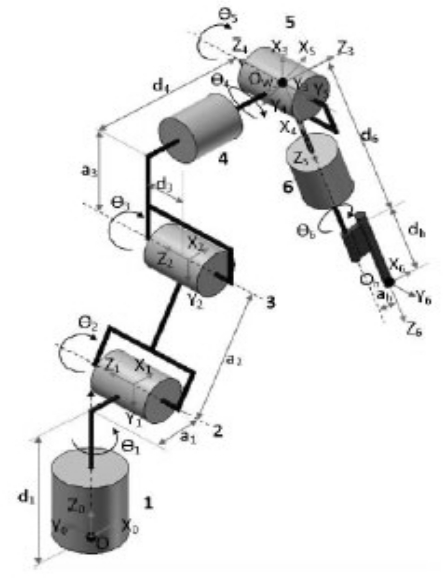
\includegraphics[width=4.5cm, height=6.5cm]{/esquema_serial.jpg}
				\caption{Esquema de sistemas de referencia en robot antropomórfico de seis grados de libertad.}
			\end{SCfigure}


		\subsection{Cinemática directa}
			El problema de la cinemática directa consiste en determinar la posición del efector final en el espacio dado el valor de cada una de las articulaciones. El valor de los ángulos de las articulaciones se determinan con ayuda de sistemas de refencia ubicados en cada una de las articulaciones del robot.\\

			Un robot manipulador está compuesto de un conjunto de enlaces conectados por varias juntas. Las articulaciones pueden ser muy simples, tales como una articulación de revolución o una articulación prismática. Una articulación de revolución es como una bisagra y permite una rotación relativa alrededor de un solo eje coordenado; una junta prismática permite un movimiento lineal a lo largo de un solo eje. En ambos casos podemos observar el que la articulación tiene un solo grado de libertad de movimiento: el ángulo de rotación en el caso de una articulación de revolución, y la cantidad de desplazamiento lineal en el caso de una articulación prismática.\\

			Con el supuesto de que cada articulación tiene un solo grado de libertad, la acción de cada una de las aticulaciones se puede describir por un solo número real: el ángulo de rotación en el caso de una articulación de revolución o el desplazamiento en el caso de una junta prismática. El objetivo del análisis de la cinemática directa es determinar el efecto acumulativo de todo el conjunto de variables de la articulación y observarlo en el efector final.\cite{spong2008robot}\\

			El análisis cinemático de un manipulador de n-enlaces puede ser extremadamente complejo y las convenciones que se presentan a continuación simplifican el análisis considerablemente.\\

			Un robot manipulador con n grados de libertad tendrá por consecuencia n articulaciones. Se numeran las articulaciones de 1 a n, y se numeran los enlaces de 0 a n, comenzando desde la base en un sistema de referencia fijo. Para esta convención, la articulación i conecta el enlace i - 1 al enlace i.\\

			Cuando se acciona la articulación i el enlace se mueve, por lo tanto, el enlace 0 (el primer eslabón) es fijo, y no se mueve cuando las juntas consecuentes son accionadas. Por supuesto, el robot manipulador podría ser móvil (por ejemplo, podría ser montado en una plataforma móvil o en un vehículo autónomo), pero para esta primer parte abordaremos el problema suponiendo una plataforma fija.\\




%%  Imagenes RGD y Points Clouds
%%  ----------------------------------------------
	\section{Imágenes RGB-D}
		En la robótica de servicios resulta imprescindible contar con robots que sean capacez de percibir su entorno, los elementos que los rodean y determinar características de los mismos. Los humanos, dadas estas necesidades, hemos desarrollado el sentido de la vista que nos permite determinar características del entorno y de los objetos que lo componen tales como el color, la forma, las dimensiones ó su ubicación en el espacio.\\

		Para optimizar los movimientos de un robot, no sólo se debe identificar cada objeto que se encuentra en el entorno de trabajo, sino también la posición que estos guardan respecto al robot. Normalmente, la segmentación de objetos de una imagen se logra mediante la segmentación de color, esta segmentación se logra a partir del análisis cromático de los componentes RGB de la imagen obtenida del objeto; sin embargo, este método es poco eficiente debido a que es sumamente suceptible a los cambios en la iluminación. \cite{objectDetectingKinect}\\ 

		Por lo tanto, necesitamos considerar una fuente de datos adicional, en este caso la profundidad, para discriminar objetos que no están en el rango de interés. En este documento se reportan los datos obtenidos al resolver este problema con la incorporación de un sensor RGB-D.\\

		La rápida evolución de esta reciente tecnología ha resultado en el aumento de la calidad de las imágenes, la mejora en la sincronización del color con la profundida y la disminución del tiempo de muestreo entre cada imagen. En partícular, la profundida de la imagen se obtiene en una matriz resultado de la proyección de rayos infrarrojos sobre los objetos. El sensor cuenta con una cámara infrarroja que obtiene la lectura de los haces infrarrojos reflejados sobre los objetos.\\

		El sensor Kinect incorpora un sensor de profundidad, un cámara de color y un arreglo de cuatro microfonos que, en conjunto, proporcionan una captura de movimiento de cuerpo completo en 3D. La figura 2.5 muestra la disposición del proyector de infrarrojos (IR), la cámara de color y la cámara IR. El sensor de profundidad consta de un proyector IR combinado con una cámara IR, la cual es un sensor semiconductor de metal-óxido monocromático. El sensor de profundidad es desarrollado por la companía israeli PrimeSense.\\

		Aunque la tecnología exacta es cerrada, se basa en el principio de la estructura de la luz y su difracción. El proyector IR es un lasér IR que pasa a traves de una rejilla de difracción y se esparce como una nube de puntos. Dada la geometría de construcción entre el proyector IR y la cámara IR se puede reconstruir un modelo 3D si se observa un punto en el proyector y posteriormente se ubica su corresponsiente reflexión en la cámara, esto se puede lograr utilizando triangulación.\\

		Debido a que el patrón de puntos es relativamente al azar, la coincidencia entre la imagen IR y el patrón del proyector puede realizarse de forma directa comparando pequeñas vecindades utilizando, por ejemplo, referencias cruzadas.\cite{kinectFeatures}\\

		El valor de la profundidad se codifica en escala de grises, cuanto más oscuro sea un píxel, más cerca está el punto de la cámara en el espacio, los píxeles negros indican que no se posee información respecto a la distancia en ese píxel. Esto puede suceder si los píxeles están demasiado lejos o demasiado cerca de la cámara IR.\\

		\begin{figure}

			\begin{subfigure}[t]{.5\textwidth}
			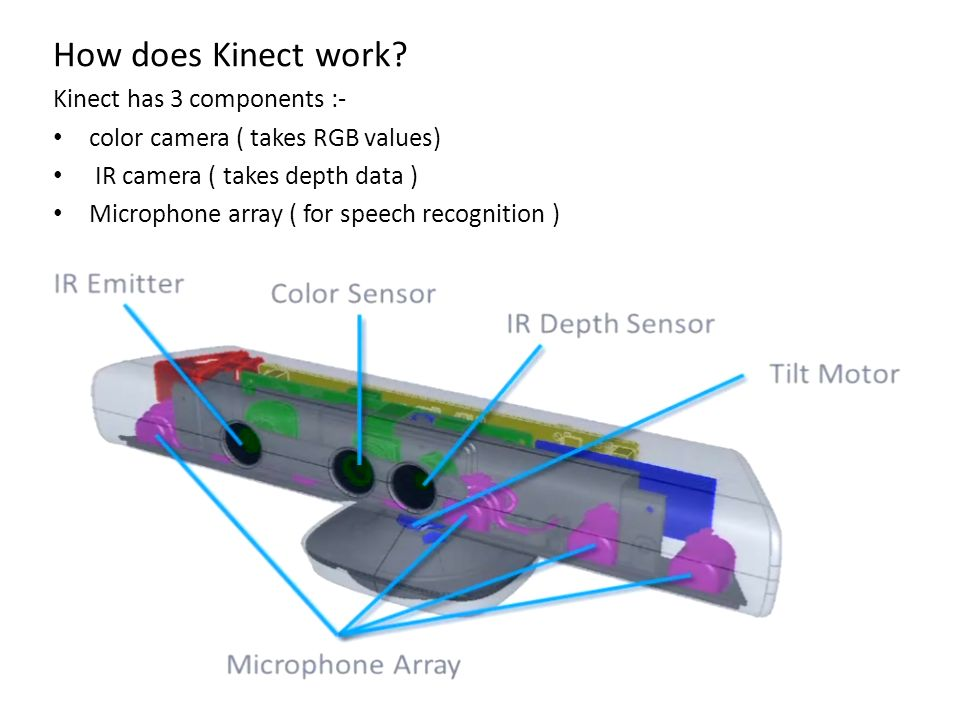
\includegraphics[width=5.5cm, height=3.0cm]{/kinect.jpg}	
			\caption{Sensor kinect}
			\end{subfigure}%
			\begin{subfigure}[t]{.5\textwidth}
			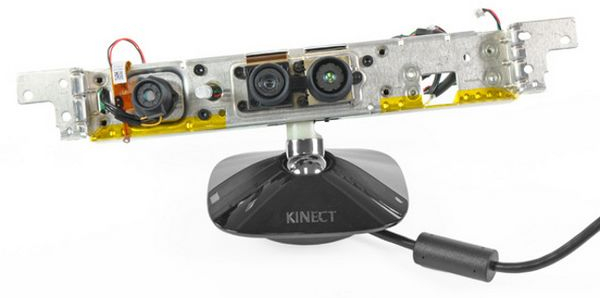
\includegraphics[width=6.5cm, height=3.0cm]{/kinect_2.jpg}
			\caption{Sensor kinect estructura}
			\end{subfigure}

			\caption{Sensor kinect elaborado por Microsoft.}

		\end{figure}

		%%\subsection{Características de las imágenes RGB-D}



	\section{Algoritmo RANSAC}
	\section{Algoritmo PCA}
	\section{Características del objeto}


	\section{Planeación de tareas}

